\documentclass{article}

% Symbols
\usepackage{amsfonts, amsthm}
\usepackage{upgreek}
\usepackage{physics}
\usepackage{cancel}
\usepackage{amssymb, latexsym, amsmath}
\usepackage{amsmath}
\usepackage{listings}

%Algorithms
\usepackage[ruled,lined,linesnumbered,commentsnumbered]{algorithm2e}

%% Identación
\setlength{\parindent}{0cm}

% Código
\newcommand{\code}[1]{\textcolor{white!25!black}{\texttt{#1}}}
\usepackage{listings}

%AMS
\usepackage{amsthm}
\newtheorem{algo-thm}{Algoritmo}

% Proof
\renewcommand*{\proofname}{\textbf{Demostraci\'on:}}

% Theorem
\newtheorem*{theorem}{Teorema}

% Hipervínculos:
\usepackage{hyperref}

% Graphics
\usepackage{graphicx}
\usepackage{pgf}

% Color a letras.
%\usepackage[usenames,dvipsnames,svgnames,table]{xcolor}

% Tikz
\usepackage{tkz-graph}
\usepackage{tikz}
\usetikzlibrary{arrows,automata}
\usepackage{tikz}
\usetikzlibrary{arrows,automata}
%\usetikzlibrary[topaths]

% Def. Dr. César.
\usetikzlibrary{shapes,calc}
\tikzstyle{edge}=[shorten <=2pt, shorten >=2pt, >=stealth, line width=1.1pt]
\tikzstyle{blueE}=[shorten <=2pt, shorten >=2pt, >=stealth, line width=1.5pt, blue]
\tikzstyle{blackV}=[circle, fill=black, minimum size=6pt, inner sep=0pt, outer sep=0pt]
\tikzstyle{blueV}=[circle, fill=blue, draw, minimum size=6pt, line width=0.75pt, inner sep=0pt, outer sep=0pt]
\tikzstyle{redV}=[circle, fill=red, draw, minimum size=6pt, line width=0.75pt, inner sep=0pt, outer sep=0pt]
\tikzstyle{redSV}=[semicircle, fill=red, minimum size=3pt, inner sep=0pt, outer sep=0pt, rotate=225]
\tikzstyle{blueSV}=[semicircle, fill=blue, minimum size=3pt, inner sep=0pt, outer sep=0pt, rotate=225]
\tikzstyle{blackSV}=[semicircle, fill=black, minimum size=3pt, inner sep=0pt, outer sep=0pt, rotate=225]
\tikzstyle{vertex}=[circle, draw, minimum size=6pt, line width=0.75pt, inner sep=0pt, outer sep=0pt]

% Margins
\addtolength{\voffset}{-1.5cm}
\addtolength{\hoffset}{-1.5cm}
\addtolength{\textwidth}{3cm}
\addtolength{\textheight}{3cm}

%Header-Footer
\usepackage{fancyhdr}
\renewcommand{\headrulewidth}{1pt}

\newcommand{\set}[1]{
  \left\{ #1 \right\}
}

%\pagenumbering{gobble} -- Este comando
%                       -- quita el número de página.
\footskip = 50pt
\renewcommand{\headrulewidth}{1pt}

\pagestyle{fancyplain}

%% Bibliografía APA
\usepackage[backend=biber]{biblatex}
\bibliography{./Bibliografia/BaseDatos}

\begin{document}
\title{UNIVERSIDAD NACIONAL AUT\'ONOMA DE M\'EXICO\\ Facultad de Ciencias}
\author{Autor: Adri\'an Aguilera Moreno}

\date{}
\maketitle
\begin{center}
  
\includegraphics[scale=0.20]{../Imagen/Portada.jpg}\\[0.4cm]
  \Large
  \bf{Lógica Computacional}
  \normalsize
\end{center}
\newpage
\fancyhead[r]{ Lógica Computacional 2022-2}
%%%%%%%%%%%%%%%%%%%%%%%%%%%%%%%%%%%%%%%%%%%%%%%%%%%%%
\section*{\LARGE{Semanal 11}}
Para cada uno de los siguientes ejercicios, \textbf{justifica ampliamente} tu respuesta.
\newline
\textbf{Desmuestra} mediante deducción natural lo siguiente:
\newcommand{\localtextbulletone}{\textcolor{black}{\raisebox{.45ex}{\rule{.6ex}{.6ex}}}}
\renewcommand{\labelitemi}{\localtextbulletone}
\begin{itemize}
\item ($a$)
  \begin{center}                                                             
    \begin{array}{rl}
      &(r \lor p) \land q \rightarrow l&
      &\;m \lor q \rightarrow s \land t&
      &(s \land t) \land l \rightarrow r&
      &\hspace*{0.5cm} p \rightarrow q&
      \hline
      &\therefore \hspace*{0.2cm} m \land q \rightarrow r&
    \end{array}
  \end{center}
  \begin{proof}
    \begin{eqnarray*}
      &1.& (r \lor p) \land q \rightarrow l \hspace*{3.4cm} \text{Premisa 1.}\\
      &2.& m \lor q \rightarrow s \land t \hspace*{3.5cm} \text{Premisa 2.}\\
      &3.& (s \land t)\land l \rightarrow r \hspace*{3.4cm} \text{Premisa 3.}\\
      &4.& p \rightarrow q \hspace*{4.7cm} \text{Premisa 4.}\\
      &5.& m \land p \hspace*{4.7cm} \text{Por la proposición 1 en la nota de clase 14.}\\
      &6.& p \hspace*{5.4cm} \text{E}_{\land} \text{ de 5.}\\
      &7.& m \hspace*{5.3cm} \text{E}_{\land} \text{ de 5.}\\
      &8.& q \hspace*{5.4cm} \text{E}_{\rightarrow} \text{ de 6 y 4.}\\
      &9.& m \lor q \hspace*{4.75cm} \text{I}_{\lor} \text{ de 7 y 8.}\\
      &10.& s \land t \hspace*{4.9cm} \text{E}_{\rightarrow} \text{ de 9 y 2.}\\
      &11.& s \hspace*{5.4cm} \text{E}_{\land} \text{ de 10.}\\
      &12.& t \hspace*{5.45cm} \text{E}_{\land} \text{ de 10.}\\
      &13.& r \lor p \hspace*{4.85cm} \text{I}_{\lor} \text{ de 6.}\\
      &14.& (r \lor p) \land q \hspace*{4.05cm} \text{I}_{\land} \text{ de 13.}\\
      &15.& l \hspace*{5.5cm} \text{E}_{\rightarrow} \text{ de 1 y 14.}\\
      &16.& (s \land t) \land l \hspace*{4.21cm} \text{I}_{\land} \text{ de 10 y 15.}\\
      &17.& r \hspace*{5.45cm} \text{E}_{\rightarrow} \text{ de 3 y 16.}
    \end{eqnarray*}
  \end{proof}
\item ($b$)
  \begin{center}                                                             
    \begin{array}{rl}
      &\hspace*{0.38cm}p \rightarrow q \lor r&
      &\hspace*{0.5cm} \neg p \rightarrow t&
      &(\neg t \lor s) \land \neg q&
      \hline
      &\therefore \;\; r \lor s&
    \end{array}
  \end{center}
  \begin{proof}
  \begin{eqnarray*}
    &1.& p \rightarrow q \lor r \hspace*{2.9cm} \text{Premisa 1.}\\
    &2.& \neg p \rightarrow t \hspace*{3.3cm} \text{Premisa 2.}\\
    &3.& (\neg t \lor s) \land \neg q \hspace*{2.4cm} \text{Premisa 3.}\\
    &4.& \neg t \lor s \hspace*{3.5cm} \text{E}_{\land} \text{ de 3.}\\
    &5.& \neg q \hspace*{4cm} \text{E}_{\land} \text{ de 3.}
  \end{eqnarray*}
  \begin{eqnarray*}
    &6.& \text{Suponemos } \neg p                                           \hspace*{4.7cm}    6.\;\; \text{Suponemos } p\\
    &7.& t \hspace*{3.2cm} \text{E}_{\rightarrow} \text{ de 6 y 2.}         \hspace*{1.65cm}   7.\;\; q \lor r  \hspace*{1.9cm} \text{E}_{\rightarrow} \text{ de 1 y 6.}\\
    &8.& s \hspace*{3.17cm} \text{E}_{\lor}       \text{ de 4 y 7.}         \hspace*{1.75cm}   8.\;\; r         \hspace*{2.4cm} \text{E}_{\lor} \text{ de 5 y 7.}\\
    &9.& r \lor s \hspace*{2.65cm} \text{I}_{\lor} \text{ de 6.}            \hspace*{2.4cm}    9.\;\; r \lor s  \hspace*{1.9cm} \text{I}_{\lor} \text{ de 8.}
  \end{eqnarray*}
  \textbf{Nota}: el paso $6$ es un supuesto, es por eso que se habré en dos, esto sería como decir
  \[p \rightarrow \bot \hspace*{2cm} p \rightarrow \top\]
  y por eso lo demuestro para ambos casos. Esto lo tenía como duda, hoy consulté y comentó la profesora que
  estaba bien siempre que en ambas partes se llegue a la conclusión que queriamos. Los pasos 8's quedan
  justificados con la demostración de abajo.
  \end{proof}
  En el ejercicio anterior se usa
  \begin{center}                                                             
    \begin{array}{rl}
      &\hspace*{0.38cm} \Gamma \vdash A \lor B&
      &\hspace*{0.5cm} \Gamma \vdash \neg A&
      \hline
      &\therefore \;\; \Gamma \vdash B&
    \end{array}
  \end{center}
  a continuación se demuestra
  \begin{center}                                                             
    \begin{array}{rl}
      &\hspace*{5cm} \text{\textbf{H.I.}}&
      \hline
      &\hspace*{1.9cm} \text{\textbf{H.I.}} \hspace*{1.7cm} \Gamma', A \vdash A \;\;\; \mathbf{(E_{\rightarrow})}&
      \hline
      &\hspace*{1.6cm} \Gamma', A \vdash A \hspace*{0.7cm} \Gamma', A \vdash \neg A \; (:= A \rightarrow \bot)  &
      \hline
      &\hspace*{2.6cm} \Gamma', A \vdash \bot  \;\; \mathbf{(E \neg)} \hspace*{2cm} \text{\textbf{H.I.}}&
      \hline
      &\Gamma' \vdash A \lor B  \hspace*{1cm} \Gamma', A \vdash B \;\;\; \mathbf{(E_{\lor})} \hspace*{1cm} \Gamma', B \vdash B \;\;\; \mathbf{(E_{\lor})}&
      \hline
      &\hspace*{2.3cm} \Gamma' = \{\Gamma, A \lor B, \neg A\}\vdash B \;\;\; \mathbf{(E_\rightarrow) \times 2}&
      \hline
      &\hspace*{1.9cm} \Gamma \vdash (A \land B) \rightarrow \neg A \rightarrow B \;\;\; \mathbf{(I_{\rightarrow}) \times 2}&
    \end{array}
  \end{center}
  Al principio me rehuse de hacer la demostración con el árbol porque tal vez pueda ser enredado, pero después de ver la demostración
  en clase (esta demostración) me quedo más claro así, aunque pasarla en LaTeX no es lo más bonito que digamos. Hice unas líneas para
  que sea más fácil seguirlo:
  \begin{center}
    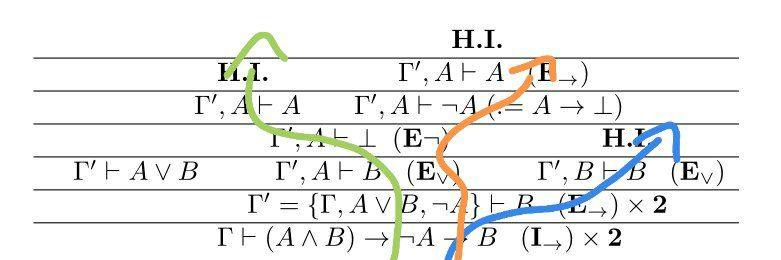
\includegraphics[scale=0.5]{./Ramificaciones.jpg}\\[0.4cm]
  \end{center}
\end{itemize}
\end{document}
